\chapter{Definición de grupos de conceptos} \label{cap:04concepto}

Para definir los grupos de conceptos es muy importante realizar la  exploración previa de las condiciones, observaciones y procedimientos  en los reportes de la base de datos (véase la sección anterior \ref{cap:03reporte} ''Reportes de la BD'').

Como en este caso, el análisis solo utiliza una fuente de datos, la base de datos S31 Registry HUVR, en la mayoría de los casos la definición de los grupos de conceptos incluye específicamente solamente los conceptos que intervienen en esta base de datos. Para estandarizar estos grupos de conceptos a cualquier base de datos y realizar el análisis en varias fuentes diferentes a la vez, bastaría con incluir también todos los descendientes de cada concepto incluído. Gracias a esta funcionalidad de ATLAS, un grupo de conceptos muy específico puede extenderse en un grupo mucho más vasto y genérico.

Por tanto, para definir los grupos de conceptos se ha seguido el siguiente procedimiento:

\begin{enumerate}
    \item \textbf{Obtener ID de los términos concretos.} Dado que un mismo concepto clínico puede expresarse con diferentes terminologías, el objetivo de esta primera tarea es identificar exactamente los términos que utiliza la base de datos.

    Para ello, se puede consultar los conceptos la base de datos directamente a través del administrador de la base de datos o se pueden visualizar a través de la herramienta \code{Data Sources} de ATLAS.

    \begin{enumerate}[label=\alph*.]
        \item \textbf{A través de pgAdmin.} Para ello ejecutamos \textit{queries} sobre la BD que devuelvan los identificadores únicos de las observaciones, condiciones y procedimientos registrados en la base de datos. Estas queries se encuentran disponibles en el repositorio de github del proyecto, en la ruta \code{Thesis-ATLAS-OHDSI/files/thesis/sql/omop\_s31\_exploration.sql}. A continuación se muestra un extracto del código.

\begin{lstlisting}[language=sql]
-- Obtiene las distintas enfermedades registradas en la BD
SELECT DISTINCT condition_concept_id FROM omop.condition_occurrence

-- Obtiene las distintas observaciones registradas en la BD
SELECT DISTINCT observation_concept_id FROM omop.observation

-- Obtiene los distintos procedimientos registrados en la BD
SELECT DISTINCT procedure_concept_id FROM omop.procedure_occurrence
\end{lstlisting}


        \item \textbf{A través de Data Source.} Para ello basta con generar los reportes de \code{Condition Ocurrence}, \code{Observation} y \code{Procedure}, tal como se realiza en la sección anterior en las Figuras \ref{figure:atlasREPORTcondition_ocurrence}, \ref{figure:atlasREPORTobservation}, \ref{figure:atlasREPORTprocedure}.
        
    \end{enumerate}

    \item \textbf{Definir un nuevo grupo de conceptos.} Una vez se conoce los términos específicos que utiliza la base de datos para nombrar los conceptos clínicos, se utiliza la herramienta \code{Concept Sets} de ATLAS para definir un nuevo grupo de concepto para cada concepto clínico en general. 

    Para la realización de este estudio se han definido 12 grupos de conceptos, tal y como muestra la Figura \ref{figure:conceptSetsCAP} ''Listado de grupos de conceptos definidos''.

\begin{figure}[H]
    \centering
    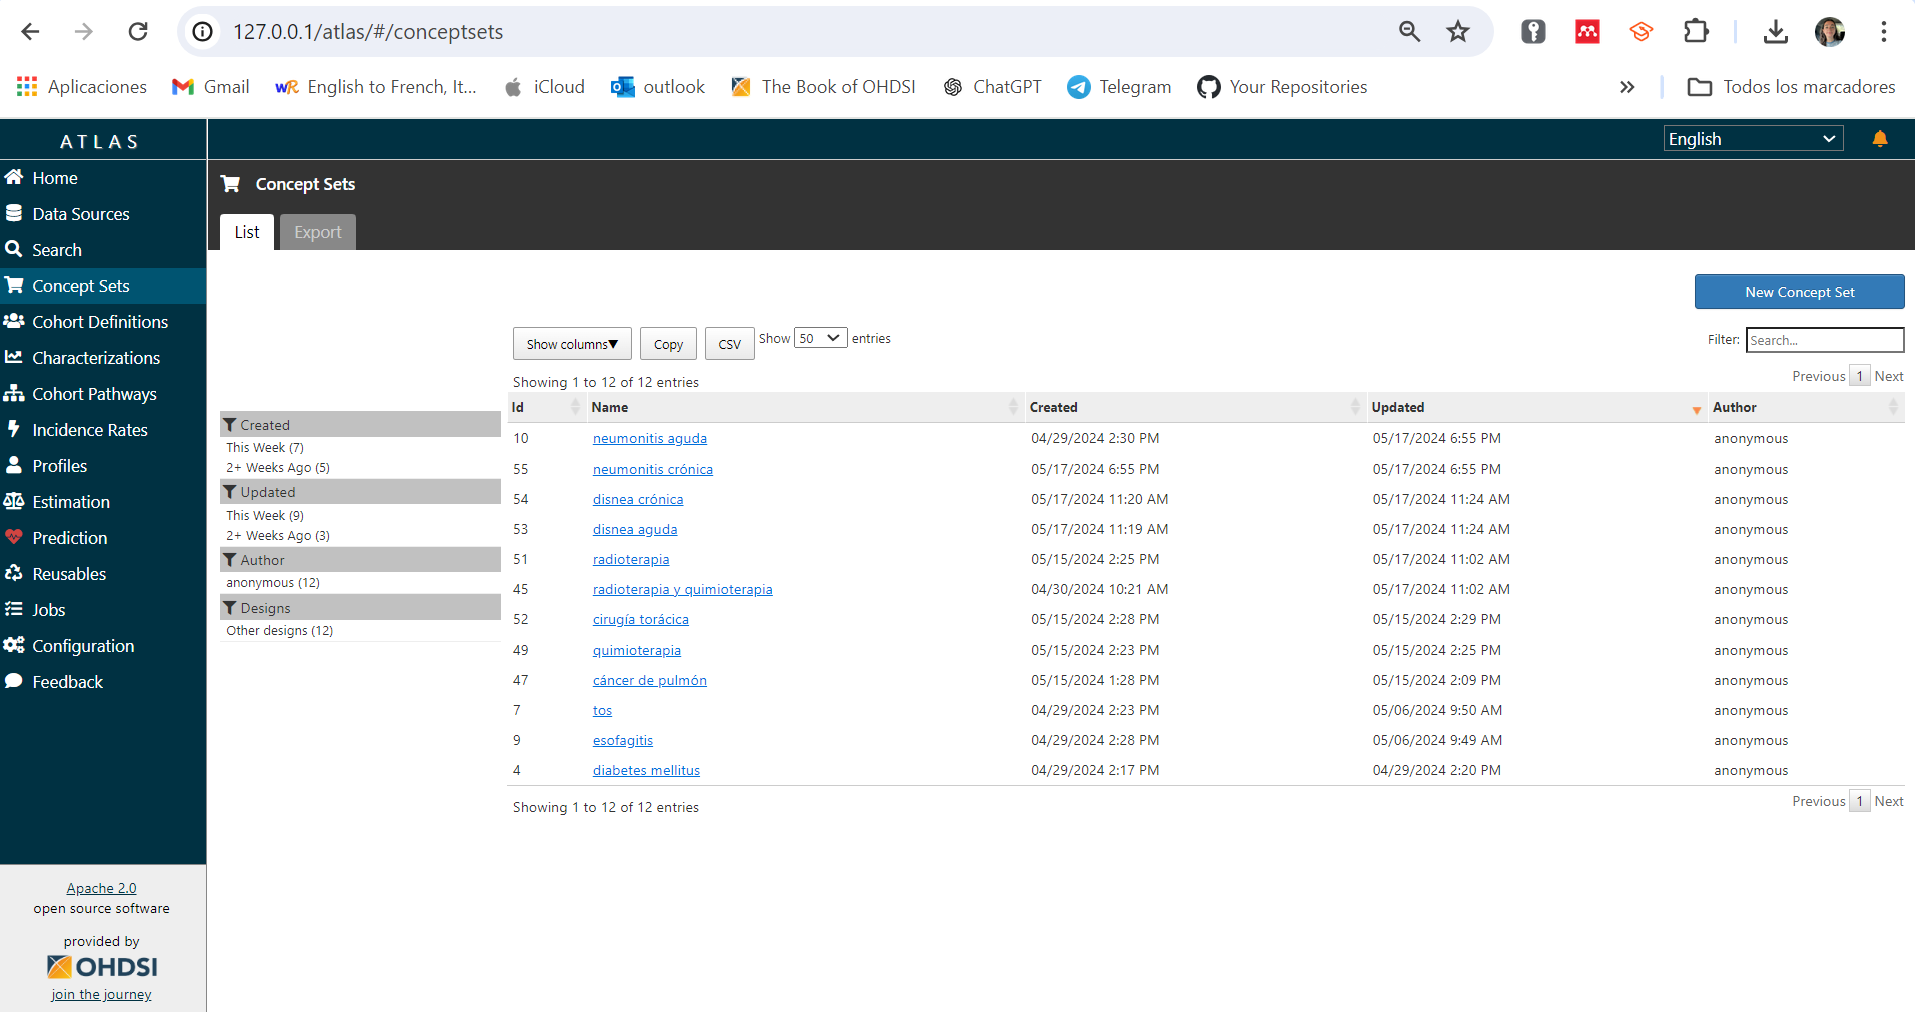
\includegraphics[width=0.90\textwidth]{figures/conceptSetsCAP.png}
    \caption{Listado de grupos de conceptos definidos}
    \label{figure:conceptSetsCAP}
\end{figure}

    \item \textbf{Exportar un grupo de conceptos.} Una vez definidos los grupos de conceptos estos se pueden exportar a formato \textbf{json} para favorecer el intercambio de información entre sistemas o la reutilización en otros estudios. ATLAS permite definir nuevos grupos de conceptos o importarlos de un archivo json, favoreciendo también la reproducibilidad del estudio. 

    A continuacións se muestra un ejemplo del formato que presentan estos conceptos una vez exportados a json.
    
\begin{lstlisting}[language=json]
{
    "ConceptSets": [
      {
        "id": 0,
        "name": "neumonitis crónica",
        "expression": {
          "items": [
            {
              "concept": {
                "CONCEPT_CLASS_ID": "Clinical Finding",
                "CONCEPT_CODE": "405569006",
                "CONCEPT_ID": 4226132,
                "CONCEPT_NAME": "Post-radiotherapy pneumonitis",
                "DOMAIN_ID": "Condition",
                "INVALID_REASON": "V",
                "INVALID_REASON_CAPTION": "Valid",
                "STANDARD_CONCEPT": "S",
                "STANDARD_CONCEPT_CAPTION": "Standard",
                "VOCABULARY_ID": "SNOMED"
              },
              "includeDescendants": true
            }
          ]
        }
      }
    ],
    "PrimaryCriteria": {
      "CriteriaList": [
        {
          "ConditionOccurrence": {
            "CodesetId": 0
          }
        }
      ],
      "ObservationWindow": {
        "PriorDays": 0,
        "PostDays": 0
      },
      "PrimaryCriteriaLimit": {
        "Type": "First"
      }
    },
    "QualifiedLimit": {
      "Type": "First"
    },
    "ExpressionLimit": {
      "Type": "First"
    },
    "InclusionRules": [],
    "CensoringCriteria": [],
    "CollapseSettings": {
      "CollapseType": "ERA",
      "EraPad": 0
    },
    "CensorWindow": {},
    "cdmVersionRange": ">=5.0.0"
  }
\end{lstlisting}


    Todos los conceptos utilizados en el proyecto se han exportado a formato json y almacenado en el repositorio de github en la ruta \code{Thesis-ATLAS-OHDSI/atlas/concept sets} para que sean accesibles públicamente.
    
\end{enumerate}